\documentclass{standalone}
\usepackage{tikz}
\usetikzlibrary{calc,positioning,fit,automata,arrows.meta,shapes.geometric}  % calc for $...$ calculations, positioning for .west .south positioning
\tikzset{
automata/.style={
every loop/.style={looseness=5},
every state/.style={very thick, fill=blue!20, draw=blue!50, text==black, ellipse},
->,>=Stealth[round], shorten >=1pt, auto, semithick,
node distance=2.8cm and 2.8cm,
font=\small,
initial text=,}}

\begin{document}
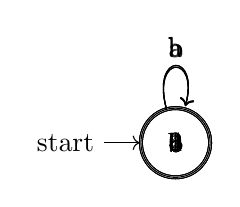
\begin{tikzpicture}
\node[state,accepting,initial] (0) {0};
\node[state,accepting] (1) {1};
\node[state] (2) {2};
\node[state,accepting] (3) {3};
\node[state] (4) {4};
%
\path (0) edge[] node[] {a} (1);
\path (0) edge[] node[] {b} (3);
\path (1) edge[loop above] node[] {a} (1);
\path (1) edge[] node[] {b} (2);
\path (2) edge[] node[] {a} (1);
\path (2) edge[loop above] node[] {b} (2);
\path (3) edge[] node[] {a} (4);
\path (3) edge[loop above] node[] {b} (3);
\path (4) edge[loop above] node[] {a} (4);
\path (4) edge[] node[] {b} (3);
\end{tikzpicture}
\end{document}
